\documentclass[border=1pt]{standalone}
\usepackage[dvipsnames]{xcolor}
\usepackage{tikz}                       % Graphen und kommutative Diagramme
\usetikzlibrary{patterns}               % Um schraffierte Formen in der tikzpicture-Umgebung zu zeichnen.

\newcommand{\ul}[1]{\underline{\smash{#1}}}
\begin{document}
\centering
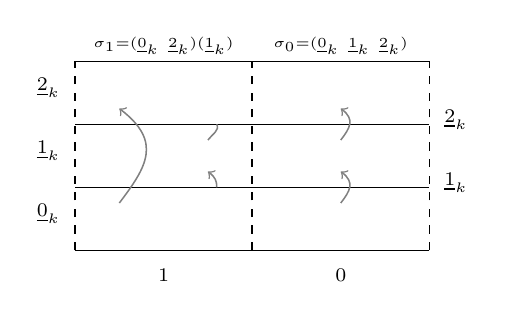
\begin{tikzpicture}[yscale=.8, xscale=2.25, line width=.55pt ]
    % Linien.
    \foreach \i in {0,...,3}
    {
        \draw[color=black] (0,\i) -- (2,\i);
    }
    \draw[color=black, dashed] (0,0) -- (0,3);
    \draw[color=black, dashed] (1,0) -- (1,3);
    \draw[color=black, dashed] (2,0) -- (2,3); 
    
    \draw[->, color=black!50] (1.5, 0.75) to[out=75, in=295] (1.5, 1.25);
    \draw[->, color=black!50] (1.5, 1.75) to[out=75, in=295] (1.5, 2.25);
    
    \draw[    color=black!50] (0.75, 1.75) to[out=75, in=280] (0.8 , 2   );
    \draw[->, color=black!50] (0.8 , 1   ) to[out=90, in=295] (0.75, 1.25);
    
    \draw[->, color=black!50] (0.25, 0.75) to[out=75, in=295] (0.25, 2.25);
    
    % Beschriftung.
    \draw node at (-.15,2.5) {$\scriptstyle\ul 2_k$};
    \draw node at (-.15,1.5) {$\scriptstyle\ul 1_k$};
    \draw node at (-.15,0.5) {$\scriptstyle\ul 0_k$};
    
    \draw node at (2.15,2) {$\scriptstyle\ul 2_k$};
    \draw node at (2.15,1) {$\scriptstyle\ul 1_k$};
    
    \draw node at (0.5,-.4) {$\scriptstyle 1$};
    \draw node at (1.5,-.4) {$\scriptstyle 0$};
    
    \draw node at (0.5,3.25) {$\scriptscriptstyle\sigma_1 = (\ul0_k\ \ul2_k)(\ul1_k)$};
    \draw node at (1.5,3.25) {$\scriptscriptstyle\sigma_0 = (\ul0_k\ \ul1_k\ \ul2_k)$};
\end{tikzpicture}

\end{document}